\documentclass[12pt]{amsart}

\usepackage[margin=0.5in]{geometry}
\usepackage{amsmath, amsthm, amssymb}
\usepackage{graphicx}
\usepackage{graphbox}
\usepackage{multicol}

\title[Derivatives Activity]{Multivariable Derivatives Activity\\Math 32}
\author[]{9/28/22}

\begin{document}

%\phantom{x}
%
%\vspace{-0.5in}

\maketitle

\begin{enumerate}
\item
\begin{enumerate}
\item
What are the names of your classmates working on this with you?

\vspace{0.5in}

\item
Are apples or oranges better, and why?
%
%\vspace{1in}
\end{enumerate}

\item
Look at the football-shaped surface.  It should be oriented like this:
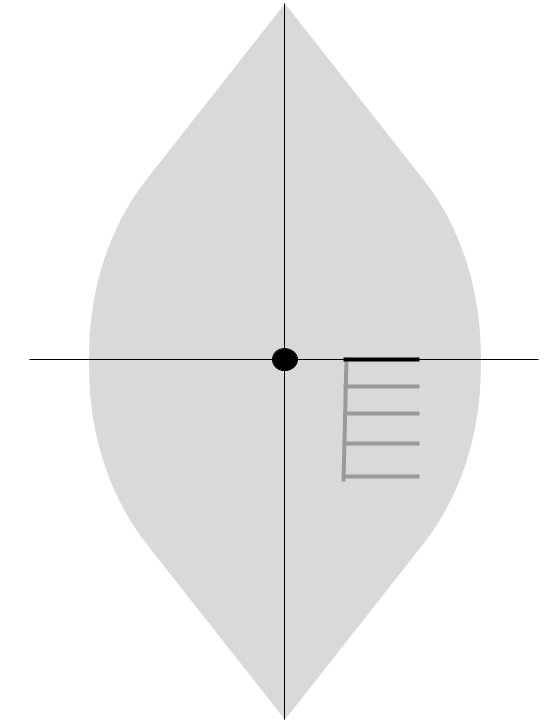
\includegraphics[height=1in]{0928-football.png}


\begin{enumerate}
\item
If the surface is given by $f(x,y)$, what  is $f_x$ at the black dot?

\vspace{0.5in}

\item
What is $f_y$ at the black dot?

\vspace{0.5in}

\item
Is $f_y$ positive or negative at the black toothpick?  How do you know?

\vspace{0.5in}

\item
Is $f_x$ positive or negative at the black toothpick?  How do you know?

\vspace{0.5in}

\item
Is $f_{yy}$ positive or negative at the black toothpick?  How do you know?

\vspace{0.5in}


\item
Is $f_{yx}$ positive or negative at the toothpick \emph{next to} the black toothpick?  How do you know?

\vspace{0.5in}




\end{enumerate}
\newpage
\item
Now, look at the half-cylinder.  Suppose the surface is given by $g(x,y)$.
\begin{multicols}{2}
\begin{enumerate}
\item
Identify all the places where $\nabla g = \vec 0$.

\bigskip
\begin{center}
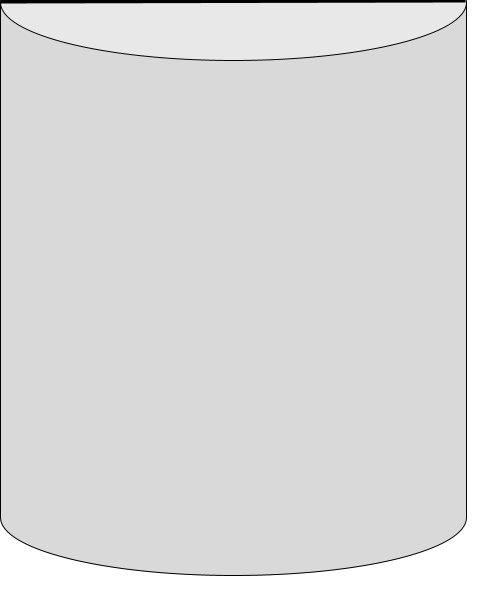
\includegraphics[height=1.5in]{0928-cylinder.png}
\end{center}

\item
Identify all the places where $\nabla g = \langle 0, a \rangle$ with $a >0$.

\bigskip
\begin{center}
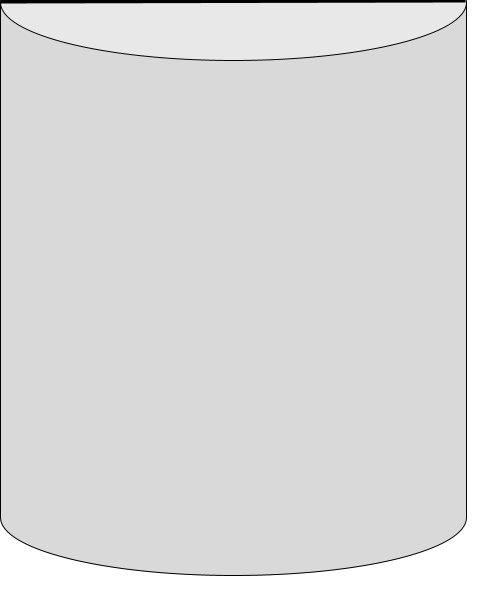
\includegraphics[height=1.5in]{0928-cylinder.png}
\end{center}

\item
Identify all the places where $\nabla g = \langle 0, a \rangle$ with $a <0$

\bigskip
\begin{center}
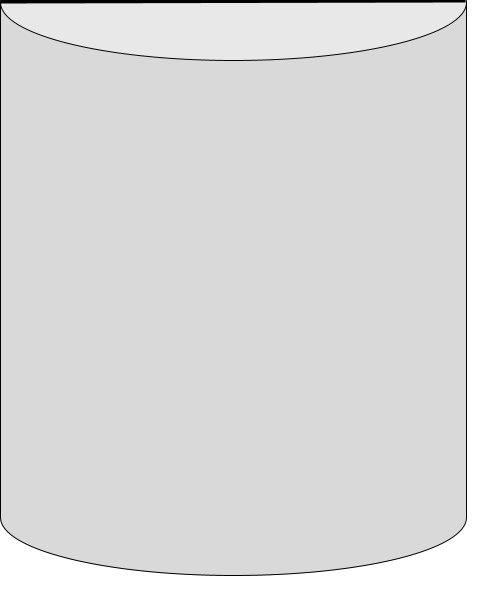
\includegraphics[height=1.5in]{0928-cylinder.png}
\end{center}

\item
Identify all the places where $\nabla g = \langle a, 0 \rangle$ with $a >0$.

\bigskip
\begin{center}
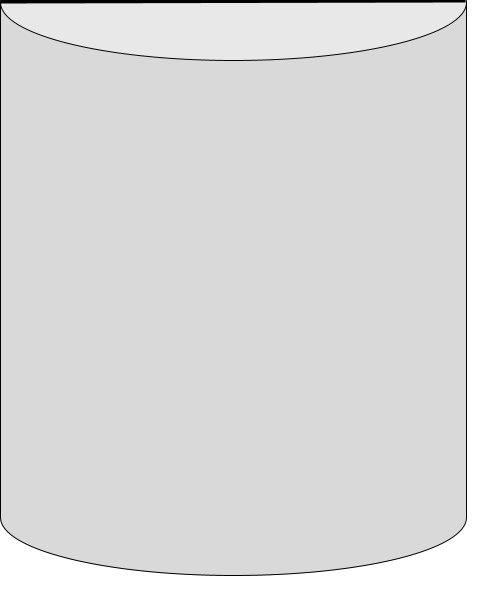
\includegraphics[height=1.5in]{0928-cylinder.png}
\end{center}

\columnbreak
\item
If $\vec v= \langle 1,1 \rangle$, identify where $D_{\vec v} g$ is positive.

\bigskip
\begin{center}
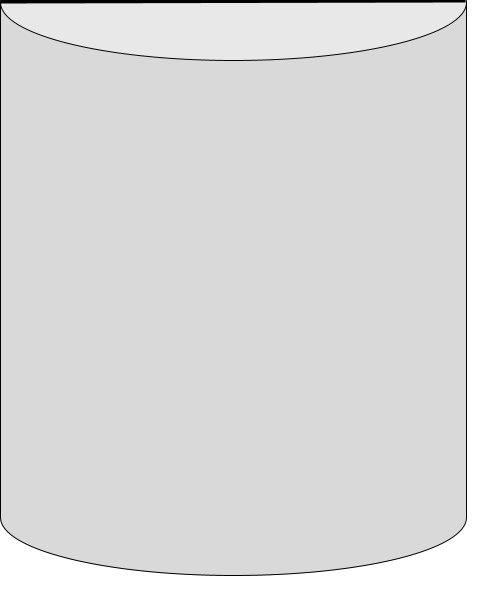
\includegraphics[height=1.5in]{0928-cylinder.png}
\end{center}



\item Find all $\vec v$ such that $D_{\vec v} g = 0$ at the black dot.
\bigskip
\begin{center}
\begin{picture}(100,100)
\put(0,0){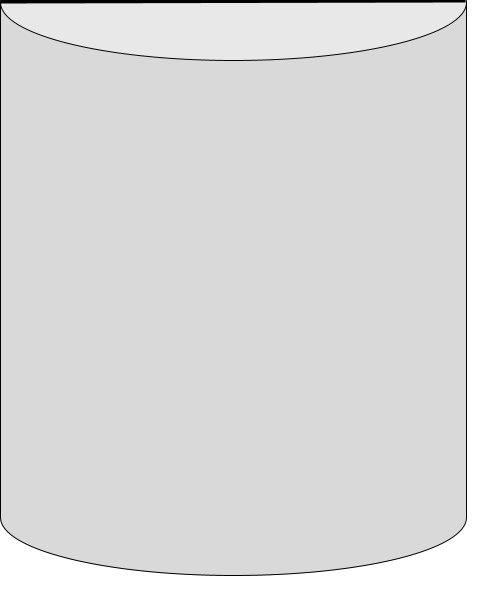
\includegraphics[height=1.5in]{0928-cylinder.png}}
\put(40,50){$\bullet$}
\end{picture}
\end{center}

\vspace{0.95in}

\item Find all $\vec v$ such that $D_{\vec v} g = 0$ at the black dot.
\bigskip
\begin{center}
\begin{picture}(100,100)
\put(0,0){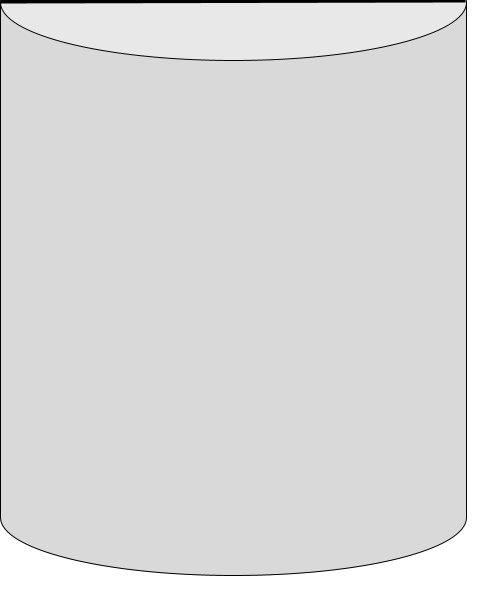
\includegraphics[height=1.5in]{0928-cylinder.png}}
\put(60,70){$\bullet$}
\end{picture}
\end{center}



\end{enumerate}
\end{multicols}

\newpage
\item
Look at exercises (2) and (3) above.  If you wanted to find the maximum of a surface, how would you be able to do it using only the fomula without graphing it?


\vspace{1in}

\item
If you finish early, confirm your answers to (2) and (3) by calculation.  The football is approximately given by
$$f(x,y) = \sqrt{1-\frac{x^2}{16} - \frac{y^2}{4}}$$
where the black dot is located near $(0,0)$ and the black toothpick is located near $(0,1)$.

The half-cylinder is approximately given by
$$g(x,y) = \sqrt{1-y^2}, \quad -2 \le x \le 2$$
where $(0,0)$ is located near the center of the surface.

Neither figure is to scale, but they do capture the general shape. 


\end{enumerate}









\end{document}